\chapter{Particules, ondes et énergie de résolution}

\section{Particules ou champs ?}

De quoi traite la physique des particules ? Des particules---mais cette réponse soulève aussitôt une question ancienne : la nature est-elle discrète ? Ici, « discret » signifie que la matière est constituée d’unités distinctes et indivisibles, et non qu’elle sait faire preuve de tact. Le mot grec \emph{atome} signifie « indivisible », bien que les objets que l’on appelle aujourd’hui des atomes puissent être décomposés. Pour l’instant, \emph{particule} sera le terme générique désignant une unité discrète.

La vision opposée est celle d’un continuum. La matière n’est alors pas un ensemble de morceaux distincts, mais une substance continue répartie dans l’espace. Son langage naturel est celui des champs. Un champ est une fonction de la position : la densité d’un matériau est un champ, tout comme les champs électrique et magnétique. Ces derniers déterminent le mouvement des particules chargées, mais, dans la conception classique, les champs eux-mêmes sont répartis continûment dans l’espace.

Il ne faut pas accorder trop d’importance à l’ordre historique de ces idées. Cette séquence est utile parce qu’elle expose la logique du raisonnement, et non parce qu’elle fournit une chronologie fiable. Le vocabulaire des particules comprend les atomes, les molécules, les collisions et les objets localisés ; celui du continuum comprend les champs et les propriétés qui varient continûment. Quelle vision est la bonne ? La mécanique quantique empêche l’une comme l’autre d’être entièrement juste, mais elle empêche aussi l’une comme l’autre d’être entièrement fausse.

La discussion sera en partie autonome, même si les raisonnements ultérieurs font appel à la mécanique quantique, à la mécanique classique, à la relativité restreinte et à l’électromagnétisme. La question immédiate est plus simple : qu’est-ce qui a d’abord convaincu les gens que la matière était réellement discrète ?

\section{Les indices chimiques en faveur d’une matière discrète}

Les premiers indices sérieux sont venus, du moins dans cette présentation logique, de la chimie plutôt que de la physique. Cette distinction est artificielle : la chimie est en grande partie la physique des atomes et des molécules. Dalton a comparé les masses d’un même nombre de molécules de différentes substances. S’assurer que les échantillons contenaient effectivement le même nombre de molécules constituait déjà un problème majeur. Le nom d’Avogadro intervient ici : une mole contient le nombre d’Avogadro de molécules. Il n’était pas nécessaire de connaître la valeur exacte de ce nombre pour comparer des échantillons contenant le même nombre de molécules.

Le résultat frappant était que les masses molaires étaient approximativement des multiples entiers de la masse molaire de l’hydrogène. Les facteurs n’étaient généralement ni \(3/2\), ni \(\pi\), ni des nombres réels quelconques, mais des nombres proches d’entiers. Le carbone-12, par exemple, représente environ douze unités de masse correspondant à celle de l’hydrogène. Cela suggère fortement une structure faite de briques élémentaires répétées, de masses presque identiques.

L’explication moderne dissipe le mystère. Les atomes ordinaires contiennent des protons, des neutrons et des électrons. La masse d’un électron ne représente qu’environ un deux-millième de celle d’un proton ou d’un neutron ; les électrons ne contribuent donc que faiblement à la masse atomique. Les protons et les neutrons en constituent presque toute la masse, et leurs masses diffèrent de bien moins d’un pour cent. Puisque le noyau de l’hydrogène ordinaire est constitué d’un seul proton, la masse d’un atome ou d’une molécule est approximativement un multiple entier d’une masse nucléaire caractéristique de l’hydrogène. Cette affirmation n’est qu’approximative : les masses du proton et du neutron ne sont pas identiques, et les électrons contribuent un peu. La quasi-intégralité de ces masses révèle néanmoins l’existence de constituants discrets.

On a ensuite compris que les molécules étaient des combinaisons d’atomes. Au dix-neuvième siècle, la chimie a identifié environ une centaine de types d’atomes et les a organisés en éléments ; dans le décompte élémentaire, environ quatre-vingt-douze sont présents dans la nature, et les isotopes introduisent d’autres distinctions. Le tableau périodique n’est pas périodique au sens naïf d’une simple répétition de blocs égaux, mais il a permis d’organiser ces espèces distinctes. À ce stade, les éléments eux-mêmes semblaient être les briques élémentaires. Les travaux d’Einstein en 1905 ont fourni une méthode quantitative permettant d’établir beaucoup plus fermement la théorie moléculaire de la matière, mais les indices chimiques avaient déjà rendu la vision atomique convaincante.

Vers la fin du dix-neuvième siècle, cette apparente conclusion a été remise en cause. On a découvert l’électron, et la radioactivité a révélé des phénomènes que la conception des éléments comme constituants élémentaires ne pouvait expliquer. À elle seule, la radioactivité contenait déjà en miniature bon nombre des questions qui allaient devenir celles de la physique nucléaire et de la physique des particules.

\section{Radioactivité et faisceaux séparés}

L’attribution exacte et la chronologie sont incertaines. Becquerel est prudemment associé à l’observation qu’un matériau radioactif, placé par hasard près d’une plaque photographique, l’avait impressionnée comme si un rayonnement invisible l’avait éclairée. Au lieu de considérer simplement la plaque voilée comme gâchée, on pouvait se demander ce qui l’avait atteinte. Les nombreux travaux ultérieurs de Marie Curie font également partie de cette histoire, mais il n’est pas nécessaire de déterminer précisément la part de chacun dans les premières découvertes pour comprendre la logique expérimentale.

Plaçons le matériau au fond d’un bloc épais de plomb et laissons un étroit canal mener à une plaque photographique. Le plomb est utile par sa forte densité, tandis que le canal collimaté permet de sélectionner ce qui s’en échappe. Au lieu d’une exposition diffuse, la plaque présente une tache localisée, ce qui suggère l’existence d’un faisceau dirigé. En ce sens, selon cette présentation logique, il s’agit du premier faisceau de particules, même si la nature du faisceau est encore inconnue.

Faisons maintenant passer le rayonnement collimaté dans un champ magnétique perpendiculaire au plan des trajectoires. L’exposition se divise en trois branches. L’une continue sans déviation. Deux autres se courbent en sens opposés, et de façon inégale. La force magnétique change de direction lorsque le signe de la charge s’inverse : les branches déviées en sens opposés se comportent donc comme des rayonnements de charges opposées, tandis que la branche rectiligne se comporte comme un rayonnement neutre.\footnote{Le schéma reconstitue le diagramme développé dans la vidéo du cours entre 00:14:34 et 00:19:31.}

\begin{figure}[h]\centering
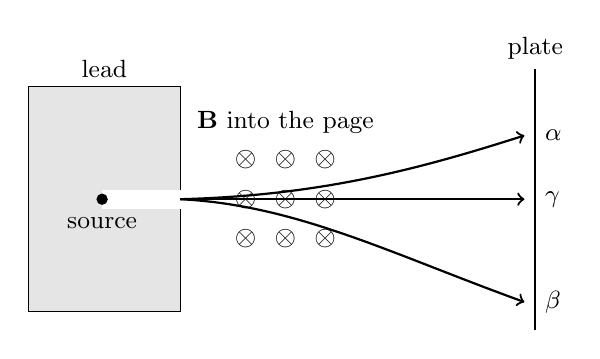
\begin{tikzpicture}[scale=0.92]
\draw[fill=gray!20] (0,-1.55) rectangle (2.1,1.55);
\draw[fill=white,draw=none] (1.02,-0.13) rectangle (2.12,0.13);
\draw[fill=black] (1.02,0) circle (0.07);
\node[below] at (1.02,-0.12) {\small source};
\node[above] at (1.05,1.55) {\small lead};
\foreach \x in {3.0,3.55,4.1}
  \foreach \y in {-0.55,0,0.55}
    \node at (\x,\y) {\(\otimes\)};
\node[above] at (3.55,0.78) {\small \(\mathbf B\) into the page};
\draw[thick] (7,-1.8) -- (7,1.8);
\node[above] at (7,1.8) {\small plate};
\draw[thick,->] (2.1,0) -- (6.85,0);
\draw[thick,->] (2.1,0) .. controls (4.0,0.05) and (5.35,0.40) .. (6.85,0.88);
\draw[thick,->] (2.1,0) .. controls (3.7,-0.08) and (5.0,-0.75) .. (6.85,-1.42);
\node[right] at (7,0.88) {\small \(\alpha\)};
\node[right] at (7,0) {\small \(\gamma\)};
\node[right] at (7,-1.42) {\small \(\beta\)};
\end{tikzpicture}\caption{Un faisceau radioactif collimaté dans un champ magnétique transverse. La composante neutre n’est pas déviée, tandis que les composantes de charges opposées se courbent en sens opposés et de façon inégale.}\end{figure}

Les trois composantes ont été nommées alpha, bêta et gamma. En termes modernes,
\begin{equation}
\begin{aligned}
\beta\text{-radiation} &= \text{electrons},\\
\alpha\text{-radiation} &= \text{helium nuclei},\\
\gamma\text{-radiation} &= \text{photons}.
\end{aligned}
\end{equation}
Une particule alpha contient deux protons et deux neutrons, ce qui explique son nombre de masse égal à quatre. Dans la séquence approximativement entière de Dalton, l’hélium aurait donc occupé la quatrième place : quatre unités nucléaires à l’échelle de l’hydrogène. Les rayons bêta sont les électrons, déjà connus grâce aux expériences sur les rayons cathodiques. Les rayons gamma ne portent aucune charge électrique.

Avec une source suffisamment diluée et un détecteur capable de distinguer les arrivées individuelles, l’exposition d’apparence continue se transforme en une succession d’événements distincts : clic, clic, clic. On peut faire de même pour les rayonnements bêta, alpha et gamma. Un compteur Geiger donne la bonne image, que les premiers appareils aient ou non été utilisés exactement dans ce régime. Chaque composante arrive sous forme de paquets discrets. Le gamma reste une énigme : il est neutre, mais on le détecte événement par événement. Le rayonnement gamma est une lumière de très haute énergie, et Planck, puis surtout Einstein, ont établi un lien entre la lumière et les quanta. Mais avant d’examiner cette conclusion, il faut prendre au sérieux les indices classiques du caractère ondulatoire de la lumière.

\section{Le caractère ondulatoire classique de la lumière}

Classiquement, la lumière était l’exemple le plus probant d’un phénomène continu. Elle est constituée de champs électrique et magnétique qui se propagent sous forme d’ondes continues. Newton avait défendu une conception corpusculaire, mais les expériences sur les ondes l’ont écartée. Une charge agitée produit un rayonnement électromagnétique. Une antenne macroscopique peut émettre des ondes radio, des micro-ondes, des infrarouges, de la lumière visible ou des ultraviolets ; une charge en mouvement à l’intérieur d’un atome joue également le rôle d’une antenne. Le rayonnement émis peut impressionner une plaque photographique.

Une ouverture unique fournit un premier indice du comportement ondulatoire. Si la lumière était un flux de projectiles, on s’attendrait à ce qu’une petite ouverture produise une tache nettement collimatée. Or l’éclairage s’étale dans une zone floue. Cet étalement ne suffit toutefois pas à trancher, car on pourrait imaginer que les particules sont déviées par des forces au bord de l’ouverture.

Deux ouvertures fournissent un test plus probant. Deux flux indépendants de particules produiraient deux taches qui se chevauchent, peut-être plus lumineuses à l’endroit de leur recouvrement. Les ondes font autre chose. Une crête issue d’une ouverture peut rencontrer la crête issue de l’autre et la renforcer ; elle peut aussi rencontrer un creux et l’annuler. L’écran présente donc une alternance de bandes claires et sombres, y compris des zones sombres que chacune des ouvertures éclairerait à elle seule.\footnote{Le schéma reconstitue les diagrammes de l’ouverture et des interférences développés dans la vidéo du cours entre 00:25:00 et 00:29:49.}

\begin{figure}[h]\centering
\resizebox{\linewidth}{!}{%
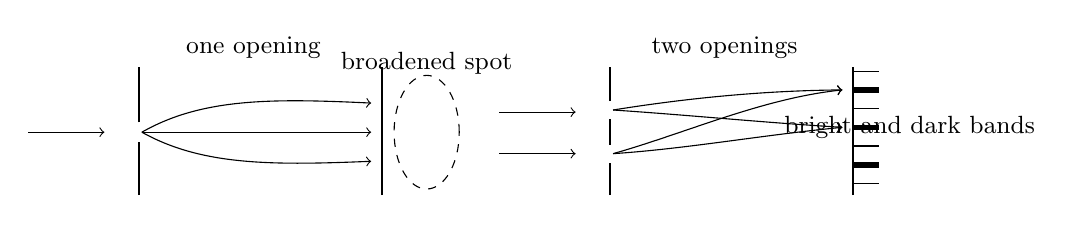
\begin{tikzpicture}[scale=0.88]
\begin{scope}
\draw[->] (-0.3,1.06) -- (0.8,1.06);
\draw[thick] (1.3,0.15) -- (1.3,0.92);
\draw[thick] (1.3,1.20) -- (1.3,2.0);
\draw[thick] (4.8,0.15) -- (4.8,2.0);
\draw[->] (1.34,1.06) .. controls (2.2,1.55) and (3.2,1.55) .. (4.65,1.48);
\draw[->] (1.34,1.06) -- (4.65,1.06);
\draw[->] (1.34,1.06) .. controls (2.2,0.58) and (3.2,0.58) .. (4.65,0.64);
\draw[dashed] (5.45,1.06) ellipse (0.47 and 0.82);
\node at (2.95,2.28) {\small one opening};
\node at (5.45,2.05) {\small broadened spot};
\end{scope}
\begin{scope}[xshift=6.8cm]
\draw[->] (-0.3,1.35) -- (0.8,1.35);
\draw[->] (-0.3,0.75) -- (0.8,0.75);
\draw[thick] (1.3,0.15) -- (1.3,0.62);
\draw[thick] (1.3,0.88) -- (1.3,1.25);
\draw[thick] (1.3,1.51) -- (1.3,2.0);
\draw[thick] (4.8,0.15) -- (4.8,2.0);
\draw[thin] (4.8,0.32) -- (5.18,0.32);
\draw[line width=2pt] (4.8,0.59) -- (5.18,0.59);
\draw[thin] (4.8,0.86) -- (5.18,0.86);
\draw[line width=2pt] (4.8,1.13) -- (5.18,1.13);
\draw[thin] (4.8,1.40) -- (5.18,1.40);
\draw[line width=2pt] (4.8,1.67) -- (5.18,1.67);
\draw[thin] (4.8,1.94) -- (5.18,1.94);
\draw[->] (1.34,0.75) .. controls (2.4,0.82) and (3.5,1.02) .. (4.65,1.13);
\draw[->] (1.34,1.38) .. controls (2.4,1.31) and (3.5,1.20) .. (4.65,1.13);
\draw[->] (1.34,0.75) .. controls (2.4,1.05) and (3.5,1.55) .. (4.65,1.67);
\draw[->] (1.34,1.38) .. controls (2.4,1.55) and (3.5,1.66) .. (4.65,1.67);
\node at (2.95,2.28) {\small two openings};
\node at (5.62,1.13) {\small bright and dark bands};
\end{scope}
\end{tikzpicture}}\caption{Une ouverture unique produit une image élargie, tandis que deux ouvertures produisent une alternance d’interférences constructives et destructives.}\end{figure}

Il est facile de se représenter le même effet avec de l’eau. Remuez la surface avec deux doigts : les ondes circulaires se propagent, se renforcent en certains endroits et s’annulent en d’autres. Ce sont les interférences, et non le simple étalement, qui constituent la signature décisive d’une onde.

Là encore, la séquence historique n’est pas simple. Dans ce schéma, Huygens est présenté avant Newton comme défenseur de la propagation ondulatoire ; Thomas Young est associé à la démonstration des interférences ; et certaines expériences d’optique de Newton lui-même se prêtent à une interprétation en termes d’interférences ondulatoires, même s’il privilégiait les corpuscules. Les expériences ultérieures sur les interférences ont établi le caractère ondulatoire de la lumière au-delà de tout doute raisonnable.

Maxwell a ensuite identifié ce qui oscille. Si une onde lumineuse se propage le long d’un axe, son champ électrique est transverse à cet axe. Son champ magnétique est lui aussi transverse et perpendiculaire au champ électrique. L’ensemble se propage à la vitesse de la lumière.\footnote{Le schéma reconstitue le diagramme de l’onde électromagnétique dessiné dans la vidéo du cours à 00:31:08.}

\begin{figure}[h]\centering
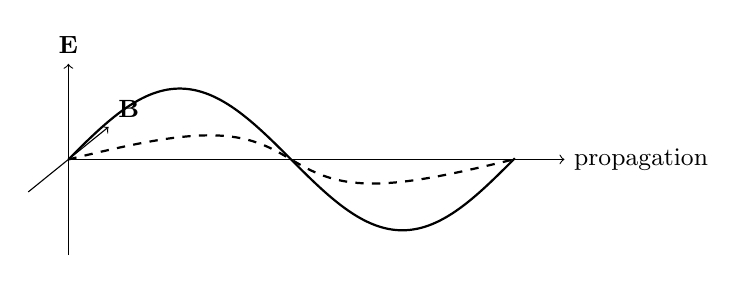
\begin{tikzpicture}[
  scale=0.9,
  x={(1cm,0cm)},
  y={(0cm,1cm)},
  z={(0.42cm,0.34cm)}
]
\draw[->] (0,0,0) -- (7,0,0) node[right] {\small propagation};
\draw[->] (0,-1.35,0) -- (0,1.35,0) node[above] {\small \(\mathbf E\)};
\draw[->] (0,0,-1.35) -- (0,0,1.35) node[above right] {\small \(\mathbf B\)};
\draw[thick,smooth,variable=\x,domain=0:6.3,samples=100]
  plot ({\x},{sin(\x r)},0);
\draw[thick,dashed,smooth,variable=\x,domain=0:6.3,samples=100]
  plot ({\x},0,{sin(\x r)});
\end{tikzpicture}\caption{Dans une onde électromagnétique, les champs électrique et magnétique sont perpendiculaires l’un à l’autre et tous deux transverses à la direction de propagation.}\end{figure}

Les oscillations de la lumière visible ordinaire sont beaucoup trop rapides pour que l’on puisse suivre directement l’alternance des champs. Pour une onde radio extrêmement longue, l’oscillation serait proportionnellement plus lente. Dans les deux cas, la même géométrie d’onde transverse produit des interférences.

\section{Longueur d’onde, période et fréquence}

La longueur d’onde \(\lambda\) est une distance spatiale : partons d’un point de l’oscillation et avançons le long de l’onde jusqu’à ce que la même phase se retrouve, après un cycle complet. Elle se mesure en mètres, en centimètres ou dans toute autre unité de longueur.

Plaçons-nous maintenant en un point et laissons passer l’onde. Le temps nécessaire pour un cycle complet est la période \(T\). La période de la lumière visible est extrêmement courte, de l’ordre de \(10^{-15}\,\mathrm{s}\) ; une longueur d’onde plus grande correspond à une période plus longue, et une longueur d’onde plus courte à une période plus courte.

Pendant une période, l’onde avance d’une longueur d’onde ; une onde de vitesse \(v\) vérifie donc
\begin{equation}
v=\frac{\lambda}{T}.
\end{equation}
Les ondes de l’eau et les ondes sonores ont leurs propres vitesses de propagation. Pour la lumière,
\begin{equation}
c=\frac{\lambda}{T}.
\end{equation}
La fréquence \(f\) est le nombre de cycles par unité de temps :
\begin{equation}
f=\frac{1}{T}.
\end{equation}
On a donc
\begin{equation}
\lambda f=c.
\end{equation}
La longueur d’onde ou la fréquence suffit à déterminer l’autre.

\begin{figure}[h]\centering
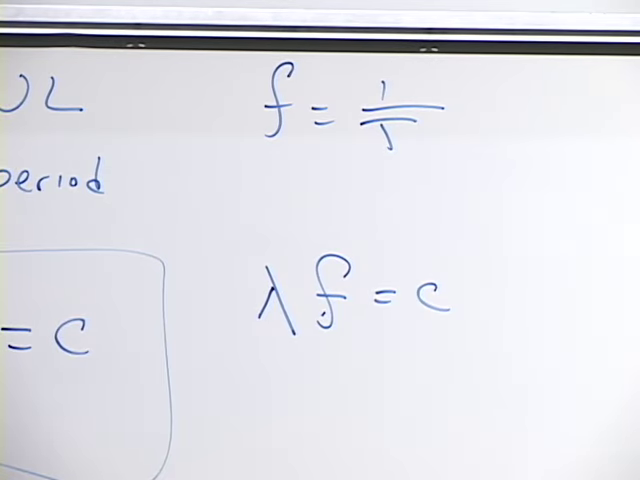
\includegraphics[width=0.68\textwidth]{lecture_01_figure_03.png}\caption{Pour une onde lumineuse, \(f=1/T\) et \(\lambda f=c\).}\lectureframe{00:36:24}\end{figure}

Les physiciens mesurent souvent le taux d’oscillation en radians par seconde plutôt qu’en cycles complets par seconde. Imaginons un mouvement uniforme sur un cercle. Si le point effectue \(f\) tours par seconde et que chaque tour compte \(2\pi\) radians, sa pulsation est
\begin{equation}
\omega=2\pi f,
\qquad
\frac{\omega}{2\pi}=f.
\end{equation}
Pour l’instant, il s’agit d’une définition ; nous reviendrons plus tard à la question pratique de savoir si elle réduit le nombre de facteurs \(2\pi\).

En combinant \(f=c/\lambda\) et \(\omega=2\pi f\), on obtient
\begin{equation}
\omega=\frac{2\pi c}{\lambda},
\qquad
\omega\lambda=2\pi c.
\end{equation}
Pour un autre type d’onde, \(c\) est remplacé par la vitesse de propagation de cette onde.

\begin{figure}[h]\centering
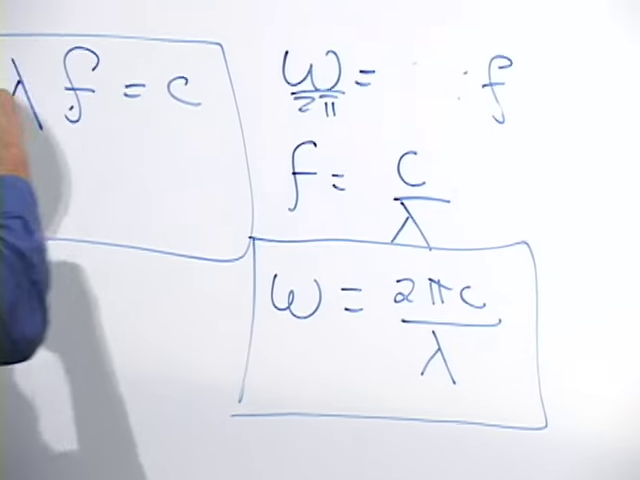
\includegraphics[width=0.68\textwidth]{lecture_01_figure_04.png}\caption{Avec \(\omega=2\pi f\), une onde lumineuse vérifie \(\omega=2\pi c/\lambda\).}\lectureframe{00:39:10}\end{figure}

Le rayonnement électromagnétique forme un spectre continu. Dans l’ordre des longueurs d’onde décroissantes, les appellations conventionnelles sont
\begin{equation}
\begin{aligned}
\text{radio}
&\longrightarrow \text{microwave}
\longrightarrow \text{infrared}
\longrightarrow \text{visible}\\
&\longrightarrow \text{ultraviolet}
\longrightarrow \text{X ray}
\longrightarrow \text{gamma ray}.
\end{aligned}
\end{equation}
La lumière visible n’occupe qu’un intervalle étroit. Les frontières entre les régions nommées sont conventionnelles ; il n’est donc pas nécessaire d’en préciser ici les longueurs d’onde de séparation. Les ondes radio peuvent être extrêmement longues ; le rayonnement gamma correspond à l’extrémité du spectre électromagnétique où les longueurs d’onde sont les plus courtes. La difficulté apparaît maintenant clairement : classiquement, le rayonnement gamma est une onde de champ continue, et pourtant il est détecté par des signaux ponctuels discrets.

\section{Arrivées discrètes et probabilités ondulatoires}

Les propriétés thermodynamiques du rayonnement ont conduit Planck et Einstein à conclure que la lumière devait être décrite en unités discrètes. Une expérience imaginaire rend cette idée frappante, mais elle ne prétend pas retracer le chemin historique réel qui a mené à cette découverte.

Éclairons un écran avec un faisceau. À intensité ordinaire, il produit une tache lumineuse d’apparence continue. Plaçons dans le faisceau un atténuateur partiellement opaque : la tache devient moins lumineuse. En augmentant plusieurs fois l’atténuation, on réduit la quantité de lumière qui arrive par unité de temps. L’apparence finit par changer. Au lieu d’une tache continûment moins lumineuse, le détecteur enregistre des événements isolés.\footnote{Le schéma reconstitue l’expérience d’atténuation développée dans la vidéo du cours entre 00:42:32 et 00:45:42.}

\begin{figure}[h]\centering
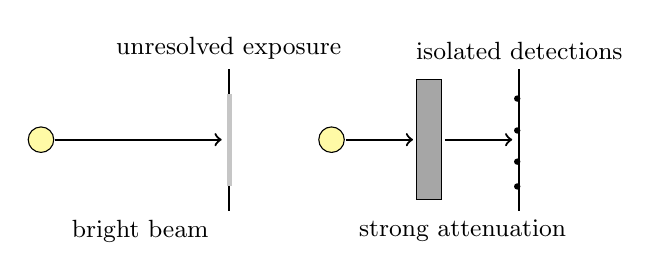
\begin{tikzpicture}[scale=0.9]
\begin{scope}
\draw[fill=yellow!35] (0,0) circle (0.18);
\draw[->,thick] (0.2,0) -- (2.55,0);
\draw[thick] (2.65,-1.0) -- (2.65,1.0);
\node[below] at (1.4,-1.0) {\small bright beam};
\end{scope}
\begin{scope}[xshift=4.1cm]
\draw[fill=yellow!35] (0,0) circle (0.18);
\draw[->,thick] (0.2,0) -- (1.15,0);
\draw[fill=gray!70] (1.2,-0.85) rectangle (1.55,0.85);
\draw[->,thick] (1.6,0) -- (2.55,0);
\draw[thick] (2.65,-1.0) -- (2.65,1.0);
\node[below] at (1.85,-1.0) {\small strong attenuation};
\end{scope}
\fill[gray!45] (2.62,-0.65) rectangle (2.70,0.65);
\foreach \y in {-0.66,-0.31,0.13,0.58}
  \fill (6.72,\y) circle (0.045);
\node[above] at (2.65,1.0) {\small unresolved exposure};
\node[above] at (6.75,1.0) {\small isolated detections};
\end{tikzpicture}\caption{Une atténuation progressive réduit le taux de détection jusqu’à ce qu’une exposition d’apparence continue se résolve en événements photoniques isolés.}\end{figure}

Si l’on attend assez longtemps, ces événements s’accumulent et forment le même profil spatial que la tache initiale. La région lumineuse était donc la somme, non résolue, de nombreuses arrivées individuelles. Cette expérience à faible intensité peut être réalisée, mais ce n’est pas l’expérience historique qui a initialement motivé l’hypothèse des photons. La proposition d’Einstein sur les photons est issue de considérations thermodynamiques et photoélectriques ; l’expérience d’atténuation donne une représentation particulièrement directe de sa conséquence.

Plaçons maintenant deux ouvertures sur le trajet du faisceau et réduisons l’intensité jusqu’à ce que les photons arrivent un à un. Chaque détection est un signal localisé. Pourtant, après de nombreuses détections, ces signaux dessinent une figure d’interférences, avec ses bandes claires et sombres. Les arrivées discrètes sont aléatoires, mais leur distribution de probabilité est celle que prédit la figure d’onde. L’onde classique devient une onde qui régit les probabilités.

L’onde et la particule ne sont donc pas deux types distincts d’entités attribués à différentes parties de la nature. Ce sont deux manifestations d’un même objet quantique. La lumière ne peut être décrite correctement comme une onde seulement ou comme une particule seulement.

Les électrons inversent la surprise initiale. On les tenait pour des particules et ils arrivent un à un au détecteur, mais, avec des ouvertures suffisamment rapprochées, ils dessinent eux aussi une figure d’interférences. Les particules alpha, environ huit mille fois plus lourdes que les électrons, obéissent au même principe, même si l’expérience est plus difficile. On a même observé des interférences avec des buckyballs : des molécules de soixante atomes de carbone disposés approximativement comme les panneaux d’un ballon de football généralisé. On s’attend à ce que le même principe s’applique même aux boules de bowling, bien qu’une telle expérience soit extraordinairement impraticable. La discussion peut s’étendre aux expériences proposées avec des virus ou des cellules vivantes, qui constituent des exemples de plus en plus ambitieux. Pour comprendre comment les descriptions ondulatoire et corpusculaire s’articulent, il faut la mécanique quantique ; la tâche immédiate consiste à extraire les propriétés du photon nécessaires à la physique des particules.

\section{Énergie du photon}

Les photons sont les éléments discrets et indivisibles de la lumière. La lumière transporte de l’énergie---la lumière du Soleil chauffe un objet qui l’absorbe---; chaque photon doit donc porter de l’énergie. Une onde monochromatique possède une longueur d’onde et une pulsation bien définies, et chacun de ses photons a
\begin{equation}
E_\gamma=\hbar\omega.
\end{equation}
Il est trompeur d’essayer de se représenter une onde continue comme un petit assemblage mécanique de points. Ce qui est bien établi, c’est la combinaison observée expérimentalement : les détections localisées suivent une distribution régie par l’onde, et l’énergie arrive en unités indivisibles.

Puisque
\begin{equation}
\omega=\frac{2\pi c}{\lambda},
\end{equation}
une longueur d’onde plus courte signifie une pulsation plus élevée, et donc davantage d’énergie dans chaque photon :
\begin{equation}
\lambda\downarrow
\quad\Longrightarrow\quad
\omega\uparrow
\quad\Longrightarrow\quad
E_\gamma\uparrow.
\end{equation}
Un seul photon radioélectrique porte très peu d’énergie. Un faisceau radio peut néanmoins transporter une énergie totale énorme parce qu’il contient un très grand nombre de photons. Pour une impulsion monochromatique contenant \(n\) photons,
\begin{equation}
E_{\text{pulse}}=n\hbar\omega,
\qquad
n=0,1,2,\ldots.
\end{equation}
L’énergie totale peut être grande, mais elle reste un multiple entier de l’énergie d’un photon.

Cette relation mène à la question pratique qui guidera la suite de la discussion. Pourquoi faut-il construire des machines toujours plus grandes pour voir des objets toujours plus petits ? Pourquoi ne pas utiliser une petite machine pour un petit objet ? La première partie de la réponse est déjà là : résoudre des structures plus petites exige une longueur d’onde plus courte, et un quantum de longueur d’onde plus courte porte davantage d’énergie.

\section{Énergie de masse au repos et masse invariante}

La physique des particules associe mécanique quantique et relativité. La relation du photon \(E_\gamma=\hbar\omega\) relève de la mécanique quantique ; le fait élémentaire correspondant en relativité est
\begin{equation}
E_{\mathrm{rest}}=mc^2.
\end{equation}
Cette précision est importante. Dans les exposés anciens, on distinguait la \emph{masse au repos} d’une \emph{masse en mouvement} dépendant de la vitesse. Dans la terminologie moderne, le terme \emph{masse} désigne la masse invariante d’un objet. Le mouvement modifie son énergie, pas sa masse. Tous les électrons ont la même masse, quel que soit leur état de mouvement, tandis que l’énergie d’un électron augmente lorsqu’on l’accélère. Ainsi, sous cette forme, \(E=mc^2\) donne l’énergie d’un objet massif dans un référentiel où l’objet dans son ensemble est au repos.

L’objet n’a pas besoin d’être immobile en son sein. Une boîte de gaz peut rester immobile sur une balance tandis que ses molécules se déplacent rapidement dans toutes les directions. L’énergie de ces mouvements internes fait partie de l’énergie de masse au repos de la boîte entière. Partons d’une boîte froide, mesurons sa masse, puis ajoutons-lui de l’énergie thermique en maintenant la boîte elle-même au repos. Sa masse au repos varie de
\begin{equation}
\Delta m=\frac{\Delta E_{\mathrm{internal}}}{c^2}.
\end{equation}
Son poids et son inertie augmentent avec sa masse. Pour une boîte ordinaire, même après une forte hausse de température, l’effet est bien trop faible pour être perceptible sur une balance ordinaire ; cette faible amplitude ne change rien au principe.

Un exemple plus frappant fait intervenir un électron et un positron. Leurs masses sont rigoureusement égales et leurs charges électriques opposées. S’ils sont initialement au repos et s’annihilent, des photons emportent l’énergie :
\begin{equation}
e^-+e^+\longrightarrow \text{photons}.
\end{equation}
L’énergie initiale est
\begin{equation}
E_{\mathrm{initial}}=2m_e c^2,
\end{equation}
et cette énergie ne peut pas disparaître. Une seule paire ne fournit qu’une quantité infime d’énergie ; il faudrait donc un nombre immense de paires pour chauffer ne serait-ce qu’une tasse de café. Mais les événements d’annihilation individuels montrent directement cette conversion.

Pour un objet au repos, masse et énergie sont donc une même grandeur physique exprimée dans des unités différentes. Le facteur \(c^2\) est le facteur de conversion entre les unités usuelles de masse et d’énergie, tout comme un facteur numérique convertit les mètres en centimètres.

\begin{classroomqa}\lecturetimestamp{01:04:39}\audiencequestion{La conversion de la masse en énergie libérée nécessite-t-elle un mécanisme ?}\lecturerresponse{Oui, un mécanisme physique est nécessaire, mais les lois de conservation contraignent déjà le résultat. Même avant de décrire le mécanisme microscopique de l’annihilation, l’énergie initiale de l’électron--positron doit réapparaître quelque part. La conservation de l’énergie permet donc de déterminer une partie importante de la réponse sans exposer en détail l’interaction.}\end{classroomqa}

\section{Dimensions et choix des unités}

Dans le système SI, la vitesse de la lumière est représentée par un très grand nombre et la constante de Planck par un très petit. La petitesse de cette dernière se devine déjà à partir de la relation du photon : la pulsation de la lumière visible est énorme, tandis que l’énergie d’un photon est minuscule ; dans ce système d’unités, \(E_\gamma=\hbar\omega\) exige donc que la valeur numérique de \(\hbar\) soit petite. En ordre de grandeur,
\begin{equation}
c\sim 10^8\ \mathrm{m\,s^{-1}},
\qquad
\hbar\sim 10^{-34}\ \mathrm{J\,s}.
\end{equation}
\editorialnote{Seuls les ordres de grandeur indiqués dans le cours sont conservés, car les derniers chiffres inscrits au tableau sont indistincts.}
Les unités sont essentielles : aucune de ces constantes ne se réduit à un simple nombre décimal. L’énergie a pour dimensions
\begin{equation}
[E]=M L^2 T^{-2},
\end{equation}
et, puisque \(E_\gamma=\hbar\omega\) avec \([\omega]=T^{-1}\), la constante de Planck a pour dimensions
\begin{equation}
[\hbar]=[E]T=M L^2 T^{-1}.
\end{equation}

Qualifier \(c\) de grande et \(\hbar\) de petite suppose déjà que l’on a choisi des unités. La vitesse exprimée en pieds par heure donne une valeur numérique de \(c\) différente de celle obtenue en mètres par seconde. En années-lumière par an, ou en secondes-lumière par seconde, la vitesse de la lumière vaut simplement un. Un choix coordonné des unités de masse, de longueur et de temps peut de même donner \(\hbar=1\).

Les systèmes d’unités familiers sont des conventions héritées, et non des caractéristiques privilégiées de la nature. Un mile contient 5280 pieds, un stone vaut quatorze livres, les chevaux se mesurent en mains et la puissance peut se mesurer en chevaux-vapeur. Le système métrique est plus systématique, mais ses échelles restent des choix humains. Rien, en physique fondamentale, ne distingue le mètre, la seconde ou le kilogramme.

La longueur, le temps et la masse fournissent trois choix indépendants d’unités de base :
\begin{equation}
L,\qquad T,\qquad M.
\end{equation}
On peut construire à partir d’eux les autres unités mécaniques. Les choix utiles dépendent du problème. Une masse solaire est pratique en astrophysique ; la masse du proton peut l’être en physique nucléaire ; les années-lumière et les années rendent les formules astronomiques relativistes plus compactes. Avec trois choix indépendants, on peut attribuer des valeurs numériques commodes à trois constantes dimensionnelles indépendantes. L’astrophysique, la physique atomique et la physique des particules n’ont pas besoin d’adopter les mêmes choix.

En physique des particules, deux conventions sont particulièrement utiles :
\begin{equation}
c=1,
\qquad
\hbar=1.
\end{equation}
Il n’existe pas de masse de particule aussi remarquable pour fixer l’unité restante. On pourrait déclarer que la masse du proton, du boson de Higgs ou du muon vaut un, mais cela ne ferait que privilégier un membre d’une grande famille.

Pourquoi choisir alors \(c\) et \(\hbar\) ? On pourrait d’abord répondre qu’ils apparaissent dans de nombreuses équations. Mais leur fréquence d’apparition ne suffit pas : la masse du proton apparaît elle aussi dans de nombreuses équations, tout comme la taille du proton. Ce qui distingue \(c\) et \(\hbar\), c’est leur universalité.

Les constantes \(c\) et \(\hbar\) sont de nature différente. La vitesse \(c\) impose une limite à tout objet physique : les objets massifs peuvent s’en approcher, mais ne peuvent pas être accélérés au-delà. La constante de Planck impose une contrainte à tout objet quantique au moyen de la relation d’incertitude en ordre de grandeur
\begin{equation}
\Delta x\,\Delta p\gtrsim\hbar.
\end{equation}
Aucune de ces affirmations ne privilégie une espèce particulière de particule. C’est cette universalité qui fait de \(c=1\) et \(\hbar=1\) des choix naturels de convention.

Le proton ne fournit aucune échelle universelle comparable. Ce n’est qu’un objet parmi d’autres. Fixer la masse du proton à un n’aurait pas plus de portée fondamentale que fixer à un la masse d’un atome de rubidium ; l’électron, le boson de Higgs et le muon posent le même problème.

La charge électrique suggère une autre grandeur universelle, mais, une fois que \(c\) et \(\hbar\) ont été normalisés, le couplage électromagnétique qui a une signification physique est sans dimension. Un changement d’unités peut déplacer des constantes dimensionnelles d’un terme à l’autre dans une formule électromagnétique ; il ne peut pas modifier un véritable couplage sans dimension.

La gravitation fournit une constante universelle dimensionnelle. Dans la formulation newtonienne, la norme de la force entre deux masses est
\begin{equation}
F=G\frac{m_1m_2}{r^2}.
\end{equation}
Toute masse gravite, tandis que des objets électriquement neutres ne sont pas nécessairement soumis à une force électrique. Ainsi, \(G\) possède l’universalité requise. C’est néanmoins une normalisation peu pratique pour la physique ordinaire des particules, car les forces gravitationnelles entre les particules élémentaires connues sont négligeables dans les calculs considérés.

\begin{classroomqa}
\lecturetimestamp{01:20:34}
\audiencequestion{Est-il légitime d’écarter simplement \(G\) ? À très haute énergie, les particules élémentaires pourraient ne pas obéir à la gravitation classique comme on le suppose ici.}
\lecturerresponse{Les particules individuelles réagissent bien au champ gravitationnel de la Terre : une particule isolée tombe dans ce champ. L’influence gravitationnelle d’une particule élémentaire sur une autre n’a pas été mesurée directement ; on peut donc remettre en question l’hypothèse d’universalité à cette échelle. Si l’on omet \(G\), c’est avant tout pour une raison pratique, et non absolue : la gravitation contribue de façon négligeable aux expériences et aux équations ordinaires de physique des particules.}
\end{classroomqa}

\begin{classroomqa}
\lecturetimestamp{01:22:01}
\audiencequestion{Pourrait-on choisir l’interaction électrique comme troisième convention de définition des unités, plutôt que la gravitation ?}
\lecturerresponse{Oui. On peut choisir un système d’unités électromagnétiques dans lequel la charge électrique, ou la constante de la loi de Coulomb, est normalisée. De telles conventions sont utilisées. Les électrons se repoussent au lieu de s’attirer, mais ce signe n’empêche pas ce choix. Ce n’est tout simplement pas la convention adoptée ici.}
\end{classroomqa}

\begin{classroomqa}
\lecturetimestamp{01:23:06}
\audiencequestion{Une fois \(c\) et \(\hbar\) fixés à un, la charge électrique est-elle sans dimension ?}
\lecturerresponse{Oui. Une grandeur sans dimension associée au carré de la charge électrique vaut approximativement \(1/137\). On peut remettre à plus tard la convention précise et l’interprétation de ce nombre ; le point essentiel ici est qu’il est sans dimension.}
\end{classroomqa}

\begin{classroomqa}
\lecturetimestamp{01:23:37}
\audiencequestion{Pourrait-on choisir la constante de Coulomb comme troisième constante à fixer à un ?}
\lecturerresponse{On peut l’absorber dans la convention d’unités électromagnétiques. Ce choix ne peut pas rendre égal à un le couplage sans dimension \(1/137\), car un changement d’unités ne modifie pas un nombre sans dimension. Aucun avantage particulier n’est revendiqué ici pour l’adoption de cette convention.}
\end{classroomqa}

\section{Équations en unités naturelles et référentiels}

Avec \(c=1\), la relation entre l’énergie de repos et la masse d’un objet massif devient
\begin{equation}
E_{\mathrm{rest}}=m.
\end{equation}
Avec \(\hbar=1\), la relation pour le photon devient
\begin{equation}
E_\gamma=\omega.
\end{equation}
On peut rétablir les constantes dès qu’on a besoin de valeurs numériques en unités conventionnelles.

\begin{figure}[h]
\centering
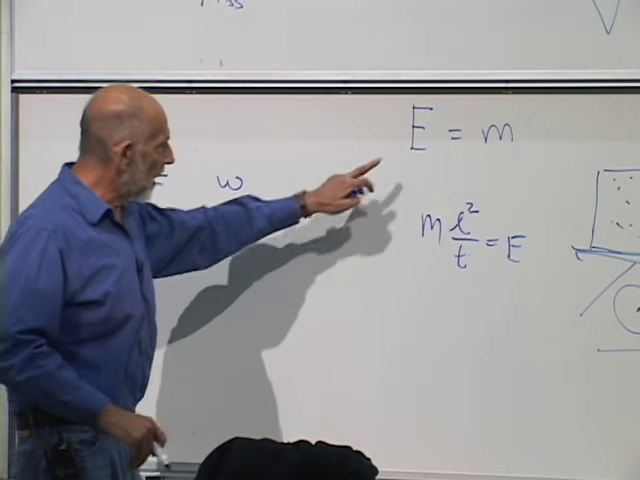
\includegraphics[width=0.72\textwidth]{lecture_01_figure_05.png}
\caption{En unités telles que \(c=1\), l’énergie de repos d’un objet massif au repos vaut \(E=m\).}
\lectureframe{01:25:40}
\end{figure}

Ces formules se ressemblent, mais elles désignent des choses différentes. Dans \(E_{\mathrm{rest}}=m\), \(E\) est l’énergie de repos d’un objet massif. Un photon n’a pas de masse et ne peut pas être mis au repos ; son énergie n’est donc pas une énergie de repos. La relation \(E_\gamma=\omega\) donne l’énergie d’un quantum sans masse en mouvement.

\begin{classroomqa}
\lecturetimestamp{01:26:07}
\audiencequestion{Que signifie \emph{au repos}, alors que le repos est toujours relatif à quelque chose et que le laboratoire lui-même n’est pas absolument au repos ?}
\lecturerresponse{Le repos se définit par rapport à un référentiel choisi. Si une tasse est immobile par rapport au laboratoire, alors, dans le référentiel du laboratoire, son énergie est égale à sa masse lorsque \(c=1\), sans contribution cinétique globale. Un autre observateur qui passe devant la tasse lui attribue également une énergie cinétique. En général, différents observateurs attribuent des énergies différentes à un même objet ou photon ; l’énergie dépend du référentiel, et il n’est pas nécessaire de supposer l’existence d’un repos absolu.}
\end{classroomqa}

On peut maintenant revenir à la convention de la pulsation. Écrire \(E_\gamma=\hbar\omega\) est compact, mais \(\omega=2\pi f\) a fait apparaître un facteur \(2\pi\) plus tôt.

\begin{classroomqa}
\lecturetimestamp{01:28:13}
\audiencequestion{Pourquoi utiliser la pulsation \(\omega\), mesurée en radians par seconde, plutôt que le nombre apparemment plus simple de cycles complets par seconde ?}
\lecturerresponse{Le choix est en partie historique, et la réponse mathématique est pragmatique plutôt qu’immédiate. La réponse proposée ici reste provisoire : écrivez les équations pertinentes une fois avec \(f\) et une fois avec \(\omega\), puis voyez quelle convention laisse apparaître le moins de facteurs \(2\pi\). Il est impossible de faire disparaître partout les facteurs \(2\pi\). Un lien possible avec la notation exponentielle complexe a aussi été évoqué, mais il n’est pas développé ici.}
\end{classroomqa}

\begin{classroomqa}
\lecturetimestamp{01:29:51}
\audiencequestion{Peut-on accélérer deux particules jusqu’à ce que leur interaction gravitationnelle mutuelle devienne importante ?}
\lecturerresponse{En principe, oui. En pratique, les accélérateurs actuels sont extrêmement loin de ce régime. La réponse dépend aussi de ce que l’on entend par particule : un corps gravitant macroscopique n’est pas le cas des particules élémentaires dont il est question ici.}
\end{classroomqa}

\begin{classroomqa}
\lecturetimestamp{01:30:27}
\audiencequestion{Quelle peut être une source de positrons ?}
\lecturerresponse{Des collisions à haute énergie peuvent créer des positrons. Certains processus nucléaires et certaines désintégrations en produisent également.}
\end{classroomqa}

\begin{classroomqa}
\lecturetimestamp{01:30:53}
\audiencequestion{Le temps de Planck et la longueur de Planck sont-ils les unités naturelles utilisées ici ?}
\lecturerresponse{Non. Les unités de Planck sont obtenues en fixant simultanément \(G\), \(c\) et \(\hbar\) à un. La longueur de Planck qui en résulte est bien plus petite que les échelles de longueur de la physique ordinaire des particules ; elle constitue donc une unité de mesure peu pratique ici. Ces unités sont naturelles lorsque gravitation, mécanique quantique et relativité interviennent toutes ensemble, comme en physique des trous noirs, en cosmologie ou en gravitation quantique. Lorsque la gravitation est négligeable, il est plus utile de fixer seulement \(c\) et \(\hbar\) à un.}
\end{classroomqa}

\section{Quantité de mouvement, lumière et résolution}

Le prochain concept fondamental est la quantité de mouvement. Un objet au repos n’a pas de quantité de mouvement, bien que son énergie de repos \(mc^2\) soit non nulle. Dès qu’il se déplace, il possède généralement une quantité de mouvement. Lors d’une collision, la quantité de mouvement se conserve tout comme l’énergie : lorsque deux objets entrent en collision, la quantité de mouvement vectorielle totale est la même avant et après la collision. Toute grandeur soumise à une loi de conservation mérite une attention particulière.

La quantité de mouvement est un vecteur : elle pointe dans la direction du mouvement. Pour un objet non relativiste,
\begin{equation}
\mathbf p=m\mathbf v.
\end{equation}
Ce n’est pas la formule générale de la relativité, et elle ne s’applique pas directement à la lumière.

La lumière transporte néanmoins de la quantité de mouvement ainsi que de l’énergie. La poussée produite par la lumière ordinaire est si faible que sa quantité de mouvement est difficile à déceler, mais une impulsion laser intense peut transmettre une impulsion mécanique considérable. Le grand laser de Livermore, par exemple, peut pousser de la matière vers l’intérieur grâce à la quantité de mouvement transportée par son rayonnement.

Considérons une impulsion suffisamment bien collimatée pour que ses rayons se propagent presque le long d’un même axe. Un faisceau réel peut présenter une certaine divergence angulaire, certaines parties se propageant dans des directions légèrement différentes ; mais, pour un faisceau idéalement collimaté, la quantité de mouvement est dirigée le long du faisceau et a pour norme
\begin{equation}
p=\frac{E}{c},
\qquad\text{or equivalently}\qquad
E=cp.
\end{equation}
On admet ici cette relation comme un fait relativiste, sans la démontrer. La vérification dimensionnelle qui suit confirme seulement que ses unités sont celles de la quantité de mouvement ordinaire :
\begin{equation}
\left[\frac{E}{c}\right]
=
\frac{M L^2 T^{-2}}{L T^{-1}}
=
M L T^{-1}
=
[m v]
=
[p].
\end{equation}
Cette comparaison dimensionnelle n’attribue pas de masse au repos à la lumière. La masse d’un photon est nulle ; il possède une quantité de mouvement parce qu’il transporte de l’énergie et se déplace à \(c\).

La direction de \(\mathbf p\) est celle de la propagation. Il est généralement difficile d’en détecter la norme, car \(c\) apparaît au dénominateur. Un faisceau peut aisément révéler son énergie en chauffant ou en vaporisant de la matière, alors que la poussée mécanique qu’il exerce est bien plus faible. Toutefois, si son intensité est suffisante, cette poussée peut devenir importante.

Pour un photon,
\begin{align}
p_\gamma
&=\frac{E_\gamma}{c}\\
&=\frac{\hbar\omega}{c}.
\end{align}
Pour exprimer cela en fonction de la longueur d’onde, revenons soigneusement aux relations d’onde. Puisque
\begin{equation}
f\lambda=c,
\qquad
\omega=2\pi f,
\end{equation}
la relation correcte est
\begin{equation}
\omega\lambda=2\pi c,
\qquad
\omega=\frac{2\pi c}{\lambda}.
\end{equation}
Il est facile d’inverser le facteur \(2\pi\) si l’on n’écrit pas explicitement les définitions. Repartir de \(f\lambda=c\) et de \(f=\omega/(2\pi)\) permet de trancher :
\begin{equation}
\frac{\omega}{2\pi}\lambda=c
\quad\Longrightarrow\quad
\omega\lambda=2\pi c.
\end{equation}
La substitution donne alors
\begin{align}
p_\gamma
&=\frac{\hbar}{c}\frac{2\pi c}{\lambda}\\
&=\frac{2\pi\hbar}{\lambda}\\
&=\frac{h}{\lambda}.
\end{align}

\begin{classroomqa}
\lecturetimestamp{01:42:38}
\audiencequestion{Est-ce que \(2\pi\hbar\) est égal à \(h\) ?}
\lecturerresponse{Oui. Par définition, \(h=2\pi\hbar\) ; \(p_\gamma=2\pi\hbar/\lambda\) est donc équivalent à \(p_\gamma=h/\lambda\). Quelle que soit la convention choisie pour la fréquence, des facteurs \(2\pi\) réapparaissent quelque part.}
\end{classroomqa}

Plus la longueur d’onde est courte, plus la quantité de mouvement du photon est grande. Un photon radio a une très grande longueur d’onde et une quantité de mouvement minuscule. Un photon gamma a une longueur d’onde très courte et transmet une impulsion bien plus importante. Un photon n’exerce toujours qu’une faible impulsion macroscopique, mais sa quantité de mouvement est bien plus grande que celle d’un photon radio. Son énergie est également plus grande, puisque \(E_\gamma=cp_\gamma\).

Cette relation explique pourquoi l’étude d’objets plus petits exige des machines plus grandes. Une photographie prise avec des longueurs d’onde bien supérieures à la taille d’une tête humaine ne montrerait qu’une image floue. Pour distinguer les traits du visage, la longueur d’onde doit être inférieure à la taille de la tête. Pour résoudre un cheveu, elle doit être comparable à l’épaisseur du cheveu ou plus petite. Pour résoudre la structure d’un atome, la longueur d’onde de la sonde ne doit pas dépasser la taille de l’atome :
\begin{equation}
\lambda_{\mathrm{probe}}\lesssim
\text{size of the structure to be resolved}.
\end{equation}
Il faut donc des longueurs d’onde plus courtes pour résoudre des structures plus petites, et des longueurs d’onde plus courtes exigent une quantité de mouvement et une énergie plus grandes. La sonde n’a pas besoin d’être un photon : d’autres particules de haute énergie obéissent à la même relation quantique entre longueur d’onde et quantité de mouvement. Pour les produire, il faut des accélérateurs qui transmettent toujours plus d’énergie à chaque particule. Les deux relations \(p_\gamma=h/\lambda\) et \(E_\gamma=\hbar\omega\) résument le raisonnement : augmenter l’énergie de la sonde augmente sa quantité de mouvement et raccourcit sa longueur d’onde.

Tel est le schéma récurrent de la physique des particules depuis environ un siècle : énergie plus élevée, quantité de mouvement plus grande, longueur d’onde plus courte et résolution spatiale plus fine.

\begin{classroomqa}
\lecturetimestamp{01:46:57}
\audiencequestion{Existe-t-il une limite inférieure théorique à la longueur d’onde ?}
\lecturerresponse{C’est possible. On s’attend à ce qu’un phénomène nouveau apparaisse près de la longueur de Planck, mais cette réponse reste provisoire. Si la résolution spatiale atteint une limite à cette échelle, celle-ci reste environ dix-sept ordres de grandeur en dessous des distances sondées au LHC ; les expériences actuelles en sont donc encore extrêmement éloignées.}
\end{classroomqa}

Le même raisonnement suggère un lien approximatif entre la taille d’un accélérateur et l’échelle qu’il peut résoudre.

\begin{classroomqa}
\lecturetimestamp{01:48:02}
\audiencequestion{La longueur d’onde, ou la taille de la structure résolue, est-elle approximativement inversement proportionnelle à la taille de l’accélérateur ?}
\lecturerresponse{En gros, oui, à condition que les champs électriques qui accélèrent les particules et les champs magnétiques qui les guident restent fixés par l’appareil disponible. Le gradient accélérateur est le gain d’énergie par unité de longueur. Pour un accélérateur linéaire de longueur \(L\) et de gradient approximativement constant \(\mathcal G\),
\[
E_{\mathrm{beam}}\sim \mathcal G L.
\]
Aux énergies ultrarelativistes, la longueur d’onde que l’on peut résoudre est inversement proportionnelle à l’énergie ; augmenter la longueur de l’accélérateur linéaire améliore donc la résolution approximativement selon le facteur inverse correspondant. Il s’agit seulement d’une loi d’échelle heuristique, et non d’une loi exacte. Dans les machines circulaires, les particules peuvent traverser plusieurs fois le même appareil, mais les charges accélérées rayonnent lorsqu’elles suivent une trajectoire courbe et perdent de l’énergie.}
\end{classroomqa}

\begin{classroomqa}
\lecturetimestamp{01:49:47}
\audiencequestion{Quelle devrait être la taille d’un accélérateur pour atteindre l’échelle de la longueur de Planck ?}
\lecturerresponse{Selon cette estimation approximative, il devrait être environ dix-sept ordres de grandeur plus long que l’accélérateur du CERN. Il n’aurait pas la taille de l’Univers, mais serait d’une dimension à peu près galactique.}
\end{classroomqa}

\begin{classroomqa}
\lecturetimestamp{01:50:09}
\audiencequestion{Comment comparer les énergies des rayons cosmiques les plus énergétiques à celles des collisionneurs ?}
\lecturerresponse{Certains rayons cosmiques peuvent avoir une énergie dans le laboratoire bien supérieure. Pour effectuer la comparaison numérique, considérons un rayon cosmique extrême dont l’énergie dans le laboratoire est de l’ordre de \(10^{21}\,\mathrm{eV}=10^{12}\,\mathrm{GeV}\). Mais un rayon cosmique frappe une cible immobile dans le laboratoire, tandis qu’un collisionneur fait se rencontrer de front deux faisceaux énergétiques. Plus important encore, des expériences utiles exigent un flux : de nombreuses particules et de nombreuses collisions bien contrôlées. Un rayon cosmique isolé peut manquer la cible pertinente ou produire un événement dont on peut tirer peu de conclusions. Une estimation volontairement extravagante, exprimée en équivalent pétrole, évaluait à environ cent mille milliards de barils par seconde l’approvisionnement nécessaire pour faire fonctionner un accélérateur galactique utile. Elle vise à montrer que l’obtention de statistiques de collision suffisantes serait un obstacle au moins aussi sérieux que la longueur de l’accélérateur.}
\end{classroomqa}

\editorialnote{L’estimation en équivalent pétrole est incohérente dans la source. Elle est d’abord énoncée, puis répétée comme étant d’environ \(10^{14}\) barils par seconde ; une reformulation ultérieure donne \(10^{11}\) barils par seconde. Les deux ordres de grandeur sont conservés au lieu d’être réconciliés tacitement.}

Ce sont de véritables échelles de distance, et non de simples grandeurs formelles. La difficulté pratique est de savoir comment les sonder sans construire un accélérateur galactique ni lui fournir une puissance fabuleuse.

\begin{classroomqa}
\lecturetimestamp{01:52:55}
\audiencequestion{Comment comparer l’énergie du LHC à celle d’un rayon cosmique d’énergie \(10^{12}\,\mathrm{GeV}\) ?}
\lecturerresponse{Pour un projectile ultrarelativiste d’énergie dans le laboratoire \(E_{\mathrm{lab}}\) qui frappe une cible fixe de masse \(m_{\mathrm{target}}\), l’énergie dans le centre de masse suit, en ordre de grandeur, la relation
\[
E_{\mathrm{cm}}\simeq
\sqrt{2m_{\mathrm{target}}c^2E_{\mathrm{lab}}}.
\]
\editorialnote{L’expression affichée pour une cible fixe explicite la dépendance en racine carrée énoncée dans cet échange.}
À masse de la cible fixée, l’énergie utile de la collision ne croît donc que comme la racine carrée de l’énergie du projectile. Ainsi, un rayon cosmique de \(10^{12}\,\mathrm{GeV}\) correspond, en ordre de grandeur, à des faisceaux se propageant en sens opposés, d’une énergie de l’ordre de \(10^6\,\mathrm{GeV}\) par faisceau, et non de \(10^{12}\,\mathrm{GeV}\) dans chaque faisceau. Les rayons cosmiques peuvent tout de même dépasser les énergies des collisionneurs terrestres, mais leur flux très faible rend impraticables les expériences systématiques et contrôlées.}
\end{classroomqa}